\documentclass[a4paper,11pt]{article}
\usepackage[spanish]{babel}
\usepackage[utf8]{inputenc}

% Configuración páginas
\usepackage{vmargin}				% Márgenes

\usepackage{sectsty}				% Fuente de los títulos
\allsectionsfont{\normalfont \Large \scshape}

\usepackage{graphicx}				% Imágenes
\graphicspath{{images/}}

\usepackage{mathtools}				% Matematicas
\newcommand\numberthis{				% numeración en align*
	\addtocounter{equation}{1}\tag{\theequation}
}

% Configuración del título
\newcommand{\horrule}[1]{\rule{\linewidth}{#1}} 	% Horizontal rule

\title{
	\vspace{-25pt}
	\normalfont \Large \textsc{
		Modelos de Investigación Operativa,
        Ingeniería Informática\\
        Universidad de Valladolid
	}\\[10pt]
	\horrule{1pt}\\[10pt]
	\huge \textbf{
		Práctica 5
	}\\
	\horrule{1pt}
}
\author{
	\normalfont \Large Daniel González Alonso
}
\date{
	\normalfont \large \today
}

%%%%%%%%%%%%%%%%%%%%%%%%%%%%%%%%%%%%%%%%%%%%%%%%%%
\begin{document}
\maketitle

%%%% RESUMEN %%%%
\begin{abstract}
	En este documento se describen los problemas y los resultados obtenidos de la práctica 5 del tema 2 de la asignatura Modelos de Investigación Operativa de Ingeniería Informática, Universidad de Valladolid.
\end{abstract}

%%%% DESARROLLO %%%%
\section{Introducción}

Esta práctica trataba sobre problemas de P-mediana y P-centro. Para estos problemas primero se va a explicar como se han resuelto los apartados y los modelos empleados:

\begin{itemize}
\item En los problemas de P-mediana el objetivo consiste en encontrar los puntos donde se van a abrir las instalaciones asegurando que la distancia total para cubrir la demanda sea mínima. El modelo empleado para los problemas de P-mediana es el siguiente:

\begin{align*}\numberthis
   	&\textrm{Minimizar }	&& z = \sum_{i=1}^{m}{\sum_{j=1}^{n}{h_i \cdot d_{i,j} \cdot y_{i,j}}}	&& \\
   	&\textrm{Sujeto a }		&& \sum_{j=1}^{n}{y_{i,j}} = 1 					&& i=1,\ldots,m \\
    &						&& y_{i,j} \leq x_j								&& i=1,\ldots,m \ \ j=1,\ldots,n \\
    &						&& \sum_{j=1}^{n}{x_j} = P						&&				\\
	&						&& x_{j} \in \{0,1\}							&& j=1,\ldots,n \\
	&						&& y_{i,j} \in \{0,1\}							&& i=1,\ldots,m \ \ j=1,\ldots,n
\end{align*}

Donde ${h_i}$ representa la demanda del punto ${i}$, ${d_{i,j}}$ contiene las distancias del punto ${i}$ al punto ${j}$, ${P}$ es el número de instalaciones que van a ser abiertas, ${x_j}$ es la variable de decisión que indica 1 si una instalación va a ser abierta en el punto ${j}$ o 0 en caso contrario y por último ${y_{i,j}}$ es la variable de decisión que dice si el punto ${j}$ queda asignado a la instalación ${i}$ en caso de valer 1 o 0 en caso contrario.

\item En los problemas de P-centro el objetivo es minimizar el tiempo de respuesta máximo entre un punto de demanda y la instalación más cercana. El modelo empleado para los problemas de P-centro es el siguiente:

\begin{align*}\numberthis
   	&\textrm{Minimizar }	&& w											&&				\\
   	&\textrm{Sujeto a }		&& \sum_{j=1}^{n}{y_{i,j}} = 1					&& i=1,\ldots,m \\
    &						&& \sum_{j=1}^{n}{t_{i,j} \cdot y_{i,j}} \leq w 	&& i=1,\ldots,m \\
    &						&& y_{i,j} \leq x_j								&& i=1,\ldots,m \ \ j=1,\ldots,n \\
    &						&& \sum_{j=1}^{n}{x_j} = p						&&				\\
	&						&& x_{j} \in \{0,1\}							&& j=1,\ldots,n \\
	&						&& y_{i,j} \in \{0,1\}							&& i=1,\ldots,m \ \ j=1,\ldots,n
\end{align*}

Donde ${x_j}$ si instalamos en el punto ${j}$ en caso de valer 1 o 0 en caso contrario. ${y_{i,j}}$ indica si la demanda del punto ${i}$ queda cubierta por una instalación en el punto ${j}$ en caso de valer 1 o 0 en caso contrario. ${t_{i,j}}$ es el tiempo de servicio desde el punto ${i}$ hasta el punto ${j}$, ${p}$ es el número total de instalaciones que se van a abrir y por último ${w}$ es el tiempo máximo de respuesta entre un punto de demanda y su punto de respuesta más cercano.
\end{itemize}

\newpage
\section{Ejercicios}

\subsection{Práctica 5.1 (P-mediana y P-centro)}

Para este problema se nos da una matriz con las distancias entre 12 puntos de población y se nos pide resolver los problemas de P-centro y P-mediana con valores de ${P}$ entre 1 y 12:

\begin{enumerate}
\item P-mediana: Para este apartado tras resolver los problemas se nos pide calcular la distancia promedio con los distintos valores de ${P}$, la cual se calcula como el valor objetivo ${\frac{z}{\sum_{i=1}^{n}{h_{i}}}}$. También se nos pide hallar la distancia máxima de una población a su centro asignado. Este problema está resuelto en el archivo \texttt{5\_1\_p\_mediana.mos} y los datos del problema en el archivo \texttt{5\_1\_p\_mediana.dat}. Los resultados obtenidos se muestran en la siguiente tabla:

\begin{table}[!htbp]
\label{5.1_p_mediana}
\centering
\begin{tabular}{|l|l|l|}
\hline
Valor de ${P}$	& Distancia promedio  & Distancia máxima	\\ \hline
1	& 25.7946	& 48	\\ \hline
2	& 17		& 33	\\ \hline
3	& 13.1784	& 30	\\ \hline
4	& 10.1838	& 28	\\ \hline
5	& 7.80541	& 28	\\ \hline
6	& 5.85405	& 28	\\ \hline
7	& 4.03784	& 15	\\ \hline
8	& 2.87027	& 15	\\ \hline
9	& 1.97838	& 15	\\ \hline
10	& 1.13514	& 15	\\ \hline
11	& 0.324324	& 12	\\ \hline
12	& 0			& 0		\\ \hline
\end{tabular}
\caption{Resultados del problema 5.1 P-mediana}
\end{table}

\newpage
\item P-centro: Para este apartado tras resolver los problemas se nos pide calcular la distancia máxima, en este caso, al tratar del problema de P-centro, solo tenemos que mostrar el valor objetivo. El problema se encuentra resuelto en el archivo \texttt{5\_1\_p\_centro.mos} y sus datos en el fichero \texttt{5\_1\_p\_centro.dat}. Los resultados obtenidos se muestran en la siguiente tabla:

\begin{table}[!htbp]
\label{5.1_p_centro}
\centering
\begin{tabular}{|l|l|}
\hline
Valor de ${P}$	& Distancia máxima	\\ \hline
1	& 47	\\ \hline
2	& 33	\\ \hline
3	& 22	\\ \hline
4	& 21	\\ \hline
5	& 19	\\ \hline
6	& 18	\\ \hline
7	& 15	\\ \hline
8	& 15	\\ \hline
9	& 12	\\ \hline
10	& 12	\\ \hline
11	& 12	\\ \hline
12	& 0		\\ \hline
\end{tabular}
\caption{Resultados del problema 5.1 P-centro}
\end{table}
\end{enumerate}

\subsection{Práctica 5.2 de P-mediana}

Para este problema se nos pide resolver los problemas de los ficheros de datos \texttt{aint1.dat} y \texttt{aint5.dat} con un valor de ${P=5}$ mediante \textit{Xpress Mosel} en NEOS Server. Los resultados obtenidos fueron los siguientes:

\begin{itemize}
\item Para el fichero de datos \textit{aint1} (${n=22}$, ${m=356}$) resuelto en el fichero \texttt{5\_2\_aint1.mos}, con ${P=5}$ el valor obtenido para ${z}$ fue de ${1.49545\mathrm{e}{+7}}$.

\item Para el fichero de datos \textit{aint5} (${n=19}$, ${m=328}$) resuelto en el fichero \texttt{5\_2\_aint5.mos}, con ${P=5}$ el valor obtenido para ${z}$ fue de ${9.84719\mathrm{e}{+6}}$.
\end{itemize}

\subsection{Páctica 5.3 de P-mediana}

Para este problema se nos da de datos los fichero \texttt{coordenadas\_15.dat}, el cual contiene las coordenadas en el eje X y en el eje Y de 15 puntos así como sus respectivas demandas ${h_i}$. Con estos datos se nos pide calcular mediante la P-mediana la distancia total, la distancia promedio y la gráfica con la asignación para los valores de ${P}$ entre 1 y 5.

Este problema se ha resuelto mediante \textit{Xpress Mosel} en el fichero ${5\_3.mos}$. Para poder resolver este problema lo primero que se ha hecho ha sido una inicialización de los datos y el posterior calculo de las distancias ${d_{i,j}}$ mediante la fórmula de la distancia euclídea:

\begin{equation}
d_{i,j} = \sqrt[]{(x_i - x_j)^2 + (y_i - y_j)^2}
\end{equation}

Los resultados obtenidos han sido los siguientes (las imágenes se pueden encontrar en la carpeta \texttt{./images}):

\begin{table}[!htbp]
\label{5.3}
\centering
\begin{tabular}{|l|p{2cm}|p{2cm}|p{8cm}|}
\hline
Valor de ${P}$	& Distancia total	& Distancia promedio	& Gráfico	\\ \hline
1	& ${1.33042\mathrm{e}{+6}}$	& 72.9997	&	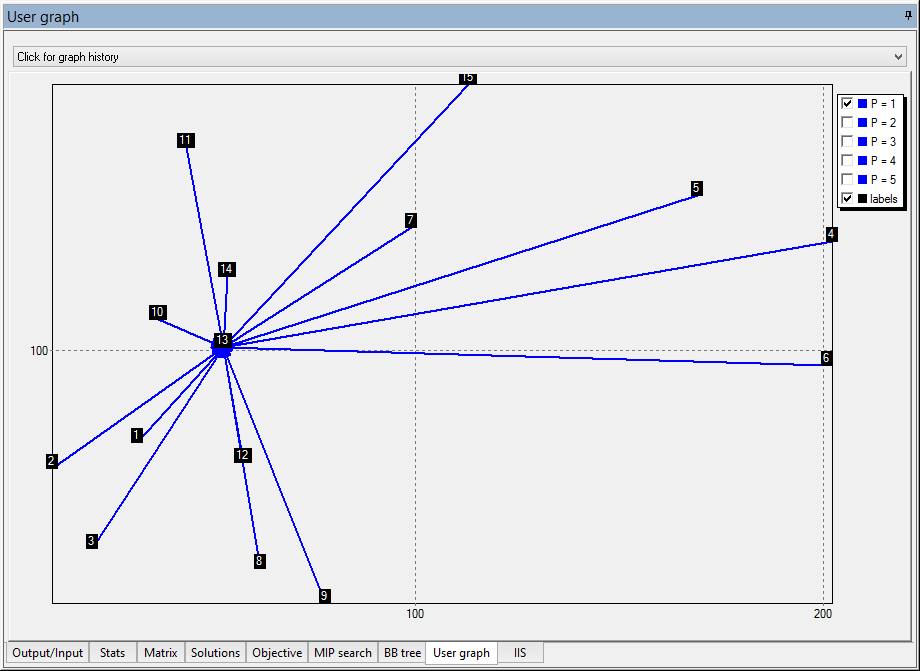
\includegraphics[width=8cm, height=4.25cm]{images/5_3_p1.png}	\\ \hline
2	& 869089	& 47.6867	& 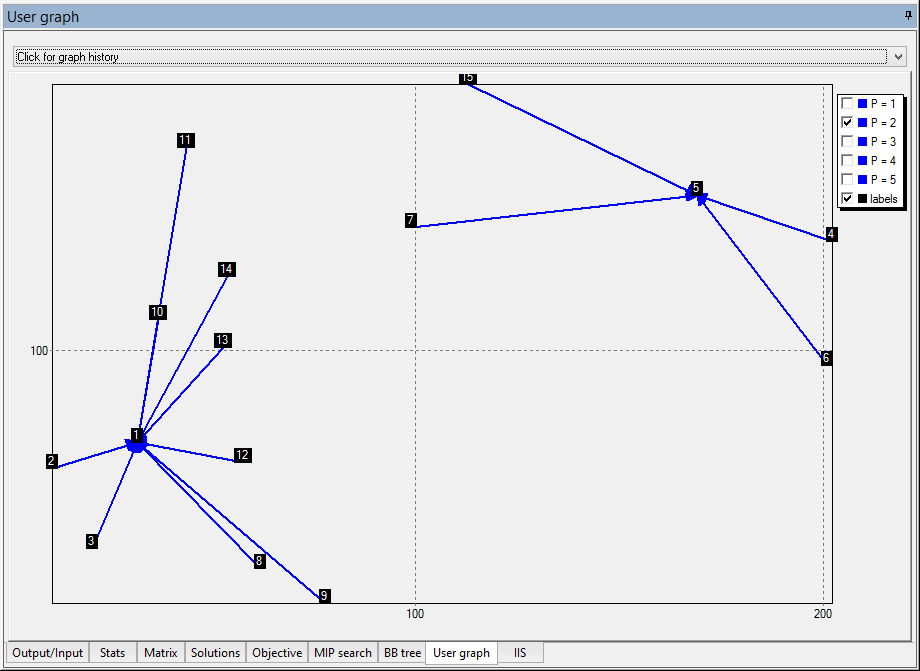
\includegraphics[width=8cm, height=4.25cm]{images/5_3_p2.png}	\\ \hline
3	& 643283	& 35.2967	& 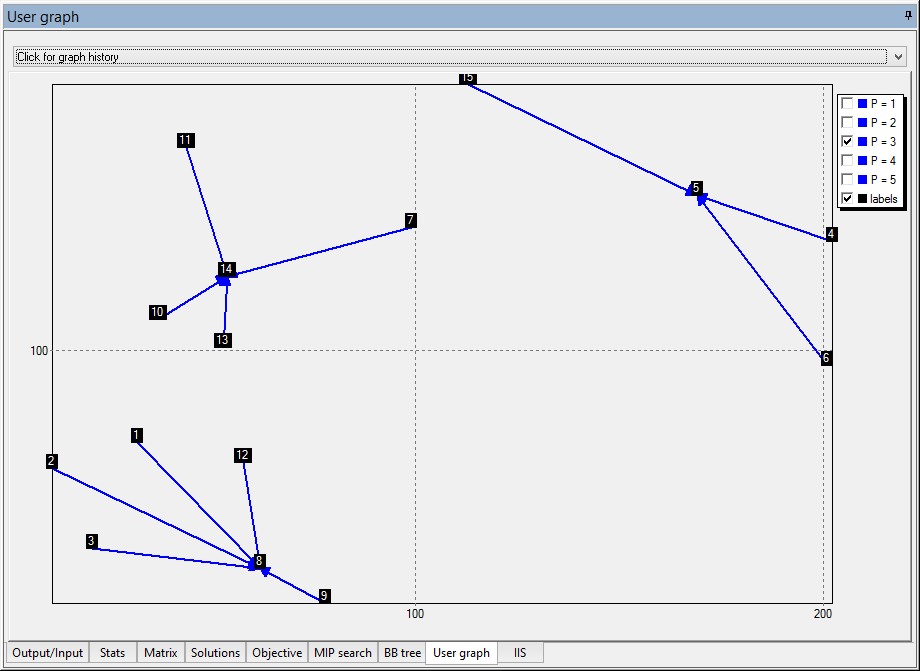
\includegraphics[width=8cm, height=4.25cm]{images/5_3_p3.png}	\\ \hline
4	& 513316	& 28.1655	& 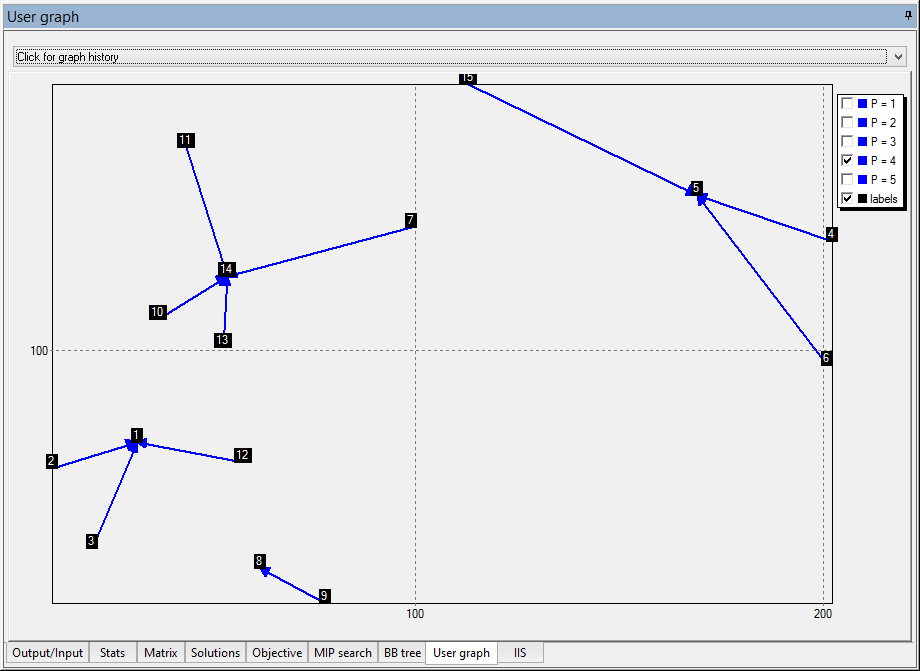
\includegraphics[width=8cm, height=4.25cm]{images/5_3_p4.png}	\\ \hline
5	& 398820	& 21.8831	& 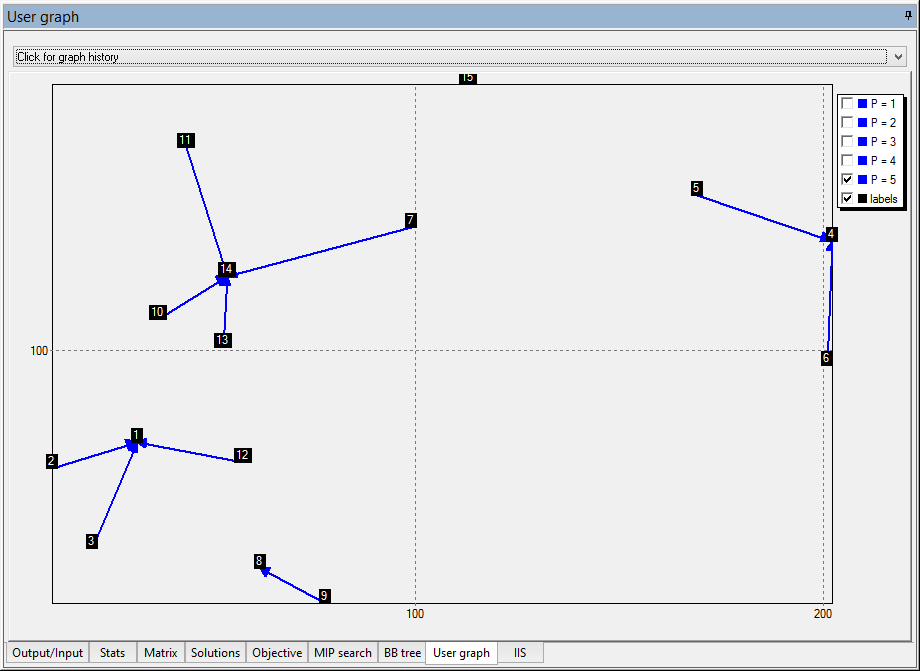
\includegraphics[width=8cm, height=4.25cm]{images/5_3_p5.png}	\\ \hline
\end{tabular}
\caption{Resultados del problema 5.3 P-mediana}
\end{table}

\begin{itemize}\item[]

\end{itemize}

\end{document}
